\documentclass{standalone}
% \usepackage[compat=1.1.0]{tikz-feynman}

\begin{document}
    \begin{subfigure}[t]{0.3\textwidth}
            \begin{tikzpicture}
                \begin{feynman}
                    \vertex (a)[dot,label=left:\(V_2\)];
                    \vertex [above left=of a] (f1) {\(1,k_4\)};
                    \vertex [above right=of a] (f2) {\(2,k_3\)};
                    \vertex [below left=of a] (i1) {\(1,k_1\)};
                    \vertex [below right=of a] (i2) {\(2,k_2\)};
                    \diagram*{
                        (i1)--[fermion](a)--[fermion](f1),
                        (i2)--[fermion](a)--[fermion](f2);
                    };
                \end{feynman}
            \end{tikzpicture}
            \caption{$V_2$ vertex}
            \label{fig:vertex2}
        \end{subfigure}
        \begin{subfigure}[t]{0.3\textwidth}
            \begin{tikzpicture}
                \feynmandiagram [horizontal=b to c, layered layout] {
                a -- [fermion,edge label'=\(2\)] b [label=below:\(V_2\)] -- [fermion, out=135, in=45, loop, min distance=3cm,edge label'=\(1\)] b -- [fermion,,edge label'=\(2\)]c,
                };
            \end{tikzpicture}
            \caption{tadpole}
            \label{fig:tadpolefromV2}
        \end{subfigure}
        \begin{subfigure}[t]{0.4\textwidth}
            \begin{tikzpicture}
                \begin{feynman}
                    \vertex (a)[dot,label=below:\(V_2\)];
                    \vertex [right=of a] (b)[dot,label=below:\(V_2\)];
                    \vertex [below left=of a] (i1) {\(1\)};
                    \vertex [below right=of b] (i2) {\(1\)};
                    \vertex [above left=of a] (f1) {\(1\)};
                    \vertex [above right=of b] (f2) {\(1\)};
                    \diagram*{
                        (i1)--[fermion](a)--[fermion](f1),
                        (i2)--[fermion](b)--[fermion](f2);
                        (a)--[fermion,out=45,in=135,edge label=\(2\)](b);
                        (b)--[fermion,out=-135,in=-45,edge label=\(2\)](a);
                    };
                \end{feynman}
            \end{tikzpicture}
            \caption{ZS for $V_1$}
            \label{fig:oneloop2}
        \end{subfigure}
        \begin{subfigure}[t]{0.3\textwidth}
            \begin{tikzpicture}
                \begin{feynman}
                    \vertex (a)[dot,label=below:\(V_2\)];
                    \vertex [right=of a] (b)[dot,label=below:\(V_2\)];
                    \vertex [below left=of a] (i1) {\(1\)};
                    \vertex [below right=of b] (i2) {\(2\)};
                    \vertex [above left=of a] (f1) {\(2\)};
                    \vertex [above right=of b] (f2) {\(1\)};
                    \diagram*{
                        (i1)--[fermion](a)--[fermion](f1),
                        (i2)--[fermion](b)--[fermion](f2);
                        (a)--[fermion,out=45,in=135,edge label=\(1\)](b);
                        (b)--[fermion,out=-135,in=-45,edge label=\(2\)](a);
                    };
                \end{feynman}
            \end{tikzpicture}
            \caption{$ZS'$ for $V_2$}
            \label{fig:oneloop3}
        \end{subfigure}
        \begin{subfigure}[t]{0.3\textwidth}
            \centering
            \begin{tikzpicture}
                \begin{feynman}
                    \vertex (a)[dot,label=below:\(V_2\)];
                    \vertex [above=of a] (b)[dot,label=below:\(V_2\)];
                    \vertex [below left=of a] (i1) {\(1\)};
                    \vertex [below right=of a] (i2) {\(2\)};
                    \vertex [above left=of b] (f1) {\(1\)};
                    \vertex [above right=of b] (f2) {\(2\)};
                    \diagram*{
                        (i1)--[fermion](a),
                        (i2)--[fermion](a),
                        (b)--[fermion](f1),
                        (b)--[fermion](f2);
                        (a)--[fermion,out=45,in=-45,edge label'=\(1\)](b);
                        (a)--[fermion,out=135,in=-135,edge label=\(2\)](b);
                    };
                \end{feynman}
            \end{tikzpicture}
            \caption{BCS for $V_2$}
            \label{bcs}
        \end{subfigure}
        \begin{subfigure}[t]{0.3\textwidth}
            \begin{tikzpicture}
                \begin{feynman}
                    \vertex (a)[dot,label=below:\(V_1\)];
                    \vertex [right=of a] (b)[dot,label=below:\(V_2\)];
                    \vertex [below left=of a] (i1) {\(1\)};
                    \vertex [below right=of b] (i2) {\(2\)};
                    \vertex [above left=of a] (f1) {\(1\)};
                    \vertex [above right=of b] (f2) {\(2\)};
                    \diagram*{
                        (i1)--[fermion](a)--[fermion](f1),
                        (i2)--[fermion](b)--[fermion](f2);
                        (a)--[fermion,out=45,in=135,edge label=\(1\)](b);
                        (b)--[fermion,out=-135,in=-45,edge label=\(1\)](a);
                    };
                \end{feynman}
            \end{tikzpicture}
            \caption{ZS with $V_1$ and $V_2$ for $V_2$}
            \label{fig:oneloop4}
        \end{subfigure}
\end{document}